%! TEX program = luatex
% ============================================================
% STANDALONE PROPOSAL — no markdown package dependency
% Requires: lualatex, uni-logo.pdf in the same directory
% ============================================================

\documentclass[a4paper,twoside]{article}

% ============================================================
% PACKAGES
% ============================================================
\usepackage{fontspec}
\usepackage[margin=1in]{geometry}
\usepackage{fancyhdr}
\usepackage[table]{xcolor}
\usepackage{amsmath,amssymb,amsfonts}
\usepackage{graphicx}
\usepackage{hyperref}
\usepackage{booktabs}
\usepackage{float}
\usepackage{tikz}
\usetikzlibrary{arrows.meta, positioning}
\usepackage{titling}
\usepackage{tocloft}
\usepackage{titletoc}
\usepackage{adjustbox}
\usepackage{etoolbox}
\usepackage[most]{tcolorbox}
\usepackage[normalem]{ulem}
\usepackage{soul}
\usepackage[none]{hyphenat}
\usepackage{titlesec}
\usepackage{datetime}
\usepackage{pgfgantt}
\usepackage{tabularx}
\newcolumntype{L}{>{\raggedright\arraybackslash}X}
\usepackage{enumitem}

\settimeformat{ampmtime}
\sloppy

% ============================================================
% COLOR DEFINITIONS (from template)
% ============================================================

% Inline Code Colors
\definecolor{inlineCodeBg}{RGB}{247,247,247}
\definecolor{inlineCodeFg}{RGB}{50,50,50}

% Quote Colors
\definecolor{quoteBg}{RGB}{247,247,247}
\definecolor{quoteBorder}{RGB}{175,175,175}

% Footnote Colors
\definecolor{footnoteRuleColor}{RGB}{150,150,150}
\definecolor{footnoteNumColor}{RGB}{150,150,150}

% ============================================================
% INLINE CODE BOX (from template)
% ============================================================
\newtcbox{\inlinecode}{
  enhanced,
  on line,
  arc=2pt,
  colback=inlineCodeBg,
  colframe=inlineCodeBg,
  boxrule=0pt,
  left=4pt,
  right=4pt,
  top=2pt,
  bottom=2pt,
  boxsep=0pt,
  before upper={\ttfamily\color{inlineCodeFg}},
}

% ============================================================
% MONOSPACE FONT (comment out if fonts/ directory is unavailable)
% ============================================================
\setmonofont{JetBrainsMonoNL}[
  Path=fonts/,
  Extension=.ttf,
  UprightFont=*-Regular,
  BoldFont=*-Bold,
  ItalicFont=*-Italic,
  BoldItalicFont=*-BoldItalic,
]

% ============================================================
% HYPERREF SETUP — clickable links & PDF metadata
% ============================================================
\hypersetup{
  pdftitle={Litho: A Template-Driven Markdown-to-LaTeX Publishing Ecosystem for Reproducible Technical Documents},
  pdfauthor={Rabia Nadeem, Abaidullah Bhatti, Abdul Rahman, Sohaib Shaukat},
  pdfsubject={Final Year Project Proposal},
  colorlinks=true,
  linkcolor=black,
  citecolor=blue!60!black,
  filecolor=magenta,
  urlcolor=cyan
}

% ============================================================
% TITLE PAGE VARIABLES
% ============================================================
\newcommand{\university}{University of Engineering and Technology}
\newcommand{\department}{Department of Computer Science}
\newcommand{\assignmenttitle}{Litho: A Template-Driven Markdown-to-LaTeX Publishing Ecosystem for Reproducible Technical Documents}
\newcommand{\assignmentsubtitle}{Final Year Project Proposal}
\newcommand{\supervisedby}{Miss Rimsha}
\newcommand{\submissioninfo}[1]{%
  \begin{tabular}{@{}ll@{}}
    #1
  \end{tabular}%
}

% ============================================================
% TITLE PAGE COMMAND
% ============================================================
\renewcommand{\maketitle}{%
  \begin{titlepage}
    \centering
    \vspace*{-1cm}

    \includegraphics[width=3cm]{uni-logo.pdf}\par
    \vspace{0.5cm}
    {\large\scshape \university\par}
    {\normalsize\scshape \department\par}
    \vspace{1.5cm}
    {\LARGE\bfseries \assignmenttitle\par}
    \vspace{0.3cm}
    {\color{gray}\rule{0.6\textwidth}{0.4pt}\par}
    \vspace{0.5cm}
    {\large{\assignmentsubtitle}\par}
    \vfill
    {
      \large
      \textbf{Submitted By}\par
      \vspace{0.3cm}
      \submissioninfo{
        Name: & Rabia Nadeem \\
        Reg\#: & 2023-CS-705 \\
        \noalign{\vspace{0.3cm}}
        Name: & Abaidullah Bhatti \\
        Reg\#: & 2023-CS-713 \\
        \noalign{\vspace{0.3cm}}
        Name: & Abdul Rahman \\
        Reg\#: & 2023-CS-725 \\
        \noalign{\vspace{0.3cm}}
        Name: & Sohaib Shaukat \\
        Reg\#: & 2023-CS-740 \\
      }
    }
    \vfill
    {
      \large
      \textbf{Supervised By}\par
      \vspace{0.3cm}
      \supervisedby\par
    }
    \vfill
    {\large Group\#: 21\par}
    \vspace{0.3cm}
    {\large Session: 2023--2027\par}
    \vspace{0.3cm}
    {\large July 31, 2026\par}
  \end{titlepage}
  \clearpage
}

% ============================================================
% TABLE OF CONTENTS STYLING (from template)
% ============================================================
\renewcommand{\cfttoctitlefont}{\Huge\bfseries\color{black}}
\renewcommand{\cftbeforetoctitleskip}{20pt}
\renewcommand{\cftaftertoctitleskip}{30pt}
\renewcommand{\cftsecfont}{\Large\bfseries\color{black}}
\renewcommand{\cftsubsecfont}{\large\color{black}}
\renewcommand{\cftsubsubsecfont}{\normalsize\color{black}}
\renewcommand{\cftsecpagefont}{\Large\color{black}}
\renewcommand{\cftsubsecpagefont}{\large\color{black}}
\renewcommand{\cftsubsubsecpagefont}{\normalsize\color{black}}
\renewcommand{\cftsecleader}{\hspace{1em}}
\renewcommand{\cftsubsecleader}{\hspace{1em}}
\renewcommand{\cftsubsubsecleader}{\hspace{1em}}
\setlength{\cftbeforesecskip}{15pt}
\setlength{\cftbeforesubsecskip}{8pt}
\setlength{\cftbeforesubsubsecskip}{5pt}

\titlecontents{section}[2em]
{\addvspace{1.2pc}\large\bfseries\color{black}}
{\contentslabel[\thecontentslabel]{2em}}
{}
{\hfill\thecontentspage}[\vspace{0.5pc}]

\titlecontents{subsection}[4em]
{\addvspace{0.8pc}\normalsize\color{black}}
{\contentslabel[\thecontentslabel]{2.5em}}
{}
{\hfill\thecontentspage}

\titlecontents{subsubsection}[6em]
{\addvspace{0.5pc}\small\color{black}}
{\contentslabel[\thecontentslabel]{3em}}
{}
{\hfill\thecontentspage}

\titlecontents{figure}[2.5em]
{\addvspace{0.8pc}\normalsize\color{black}}
{\contentslabel[\thecontentslabel]{2.5em}}
{}
{\hfill\thecontentspage}

\titlecontents{table}[2.5em]
{\addvspace{0.8pc}\normalsize\color{black}}
{\contentslabel[\thecontentslabel]{2.5em}}
{}
{\hfill\thecontentspage}

\renewcommand{\contentsname}{%
  \vspace{-20pt}%
  \centerline{\Huge\bfseries\color{black}{Contents}}%
  \vspace{15pt}%
}

% ============================================================
% LIST OF FIGURES / TABLES STYLING (matching ToC)
% ============================================================
\renewcommand{\listfigurename}{%
  \vspace{-20pt}%
  \centerline{\Huge\bfseries\color{black}{List of Figures}}%
  \vspace{15pt}%
}

\renewcommand{\listtablename}{%
  \vspace{-20pt}%
  \centerline{\Huge\bfseries\color{black}{List of Tables}}%
  \vspace{15pt}%
}

% ============================================================
% SECTION FORMATTING (from template)
% ============================================================
\titleformat{\section}
{\LARGE\bfseries}{\thesection}{1em}{}
\titleformat{\subsection}
{\Large\bfseries}{\thesubsection}{1em}{}
\titleformat{\subsubsection}
{\large\bfseries}{\thesubsubsection}{1em}{}
\titleformat{\paragraph}
{\normalsize\bfseries}{\theparagraph}{1em}{}
\titleformat{\subparagraph}
{\small\bfseries}{\thesubparagraph}{1em}{}

\titlespacing*{\section}
{0pt}{3.5ex plus 1ex minus .2ex}{2.3ex plus .2ex}
\titlespacing*{\subsection}
{0pt}{3.25ex plus 1ex minus .2ex}{1.5ex plus .2ex}
\titlespacing*{\subsubsection}
{0pt}{3.25ex plus 1ex minus .2ex}{1.5ex plus .2ex}
\titlespacing*{\paragraph}
{0pt}{3.25ex plus 1ex minus .2ex}{1em}
\titlespacing*{\subparagraph}
{0pt}{3.25ex plus 1ex minus .2ex}{1em}

% ============================================================
% ALTERNATING TABLE ROW COLORS (from template)
% ============================================================
% Removed to prevent striped design on the "Submitted By" table.

% Float default
\makeatletter
\renewcommand{\fps@table}{H}
\makeatother

% ============================================================
%                      DOCUMENT BODY
% ============================================================
\begin{document}

% ---- Title Page ----
\thispagestyle{empty}
\maketitle

% ---- Table of Contents ----
\setcounter{tocdepth}{3}
\tableofcontents
\thispagestyle{empty}
\clearpage

% ---- List of Figures ----
\listoffigures
\thispagestyle{empty}
\clearpage

% ---- List of Tables ----
\listoftables
\thispagestyle{empty}
\clearpage

% ---- Headers / Footers ----
\fancyhf{}
\fancyhead[LE,RO]{\thepage}
\fancyhead[LO,RE]{\leftmark}
\renewcommand{\sectionmark}[1]{\markboth{\thesection\ #1}{}}
\renewcommand{\subsectionmark}[1]{}
\pagestyle{fancy}
\raggedbottom

% ============================================================
%              CHAPTER 1: PROJECT OVERVIEW
% ============================================================
\section{Chapter 1: Project Overview}

% ------------------------------------------------------------
\subsection{Abstract}

Authors of technical documents -- theses, conference papers, university proposals, technical books -- face a persistent trade-off. LaTeX produces publication-quality typesetting but imposes a steep learning curve, verbose markup that clutters version-control diffs, and no separation between an institution's house style and a student's content. Word processors are approachable but store content in opaque binary-adjacent formats that resist meaningful diffs, branching, and collaborative review through standard developer tooling. Plain Markdown is universally known, plain-text, and diff-friendly, but on its own has no notion of templates, citations, captioned figures, or the extensibility a real technical document needs, leaving authors to either hand-write LaTeX anyway or accept generic, unstyled conversion output.

\textbf{Litho} is a template-driven publishing ecosystem that resolves this trade-off. Authors write in a three-tier Markdown dialect -- (1) standard Markdown, (2) an extended syntax layer covering the constructs technical documents most often need such as complex tables, highlighting and underlining, citations, mathematics, and Mermaid diagrams, and (3) a custom syntax layer defined by each individual template -- and a custom interpreter binds that content to a publisher-authored LaTeX template and compiles it to a polished PDF, with no LaTeX knowledge required from the author and no loss of git-friendly, plain-text source.

The core of this vision is already built and in daily use: the Litho compiler and command-line interface convert plain Markdown into publication-quality PDFs today, a capability many people rely on~\cite{ref7}. This very proposal document, for example, was authored in Markdown and compiled to PDF with Litho. The current build uses a single, hard-coded template; the remaining scope of this project is to generalise that hard-coded template into the first-class, pluggable template system that the rest of this proposal describes -- (1) the Litho language specification and interpreter, (2) a command-line interface for authoring and for publishing templates, (3) a Visual Studio Code extension together with companion rendering plugins for other editors' native Markdown viewers, providing syntax highlighting, snippets, and schema-aware IntelliSense for both the core syntax and any template's custom shortcodes, (4) a template marketplace, backed by Supabase, through which universities, publishers, and individual authors can share reusable templates, convert documents directly in the browser, and author new templates with AI assistance grounded in a curated template dataset, (5) an MCP server and a hosted conversion API with webhooks so AI assistants and any Markdown-based website can invoke Litho directly, and (6) full round-trip fidelity: every compiled PDF carries its original Markdown source embedded in its metadata, so the exact source can always be recovered from the output alone, with no reconstruction or guesswork involved. Section 2.1 details how this scope is sequenced and delivered within the two-semester Final Year Project timeline.

% ------------------------------------------------------------
\subsection{Introduction}

Markdown has become the default plain-text authoring format for developers: it is the format of READMEs, static-site generators, note-taking applications, and most technical documentation platforms, precisely because its syntax is minimal enough to be learned in minutes and readable even unrendered~\cite{ref1}. LaTeX, in contrast, remains the format of record for typeset technical output -- theses, journal papers, and camera-ready conference submissions -- because no other open system offers comparable control over mathematics, bibliographies, cross-referencing, and multi-column layout~\cite{ref2}.

The two formats are rarely combined well. Pandoc, the most widely used document converter, treats Markdown-to-LaTeX conversion as a best-effort, template-agnostic transformation: it can substitute values into a single LaTeX template per invocation, but it was not designed as a platform for a marketplace of interchangeable, versioned, schema-validated templates, and its Markdown dialect is not extensible with template-specific syntax that an editor can understand~\cite{ref3}. Newer systems such as Quarto and R Markdown layer publishing on top of Markdown, but they are oriented around computational notebooks for data science and still ultimately depend on Pandoc's conversion model~\cite{ref4}. Typst, released in 2019 and gaining traction as a LaTeX alternative, abandons Markdown and LaTeX syntax entirely in favor of a new markup and scripting language, which delivers fast compilation but requires authors to learn a new language from scratch and offers no path for the millions of existing Markdown-literate authors to opt in incrementally~\cite{ref5}.

Litho's position is to leave Markdown as the authoring surface -- the syntax nearly every developer and student already knows -- while treating templates as first-class, publishable, versioned artifacts, and treating editor tooling as part of the core deliverable rather than an afterthought. This mirrors how the npm registry turned JavaScript from a scripting language into an ecosystem, and how the Visual Studio Code extension API turned a text editor into an extensible platform: the goal is not a better converter, but a small language plus a marketplace plus first-class editor support, designed together from the outset.

% ------------------------------------------------------------
\subsection{Problem Statement}

A student writing a university proposal, or a researcher preparing a camera-ready paper, today has three unsatisfying options. They can write LaTeX directly, which typically means starting from a template file whose macros they do not understand and cannot safely modify. They can write in Word, which cannot be meaningfully diffed or merged with standard version-control tools and offers no clean separation between an institution's required formatting and the author's own content. Or they can write Markdown and run it through a generic converter, which renders paragraphs and headings correctly but has no way to express template-specific requirements -- a Gantt chart in a proposal, a required title-page field, a callout box, a citation style -- because plain Markdown was never designed to be extended per template, and no diff-friendly authoring text-format has a marketplace where such templates can be published, versioned, and discovered.

A second, related gap is tooling. Even where an extended syntax might exist, standard editors have no awareness of it: a VS Code Markdown preview renders an unrecognized template shortcode as broken plain text rather than the intended figure, callout, or citation, which undermines the very promise of a "what you write is close to what you get" authoring experience.

Litho addresses both gaps together: an extensible, formally specified Markdown dialect with a template-binding compiler, and first-class editor tooling that understands both the dialect's core syntax and any individual template's declared extensions.

% ------------------------------------------------------------
\subsection{Objectives}

\begin{enumerate}
  \item \textbf{Specify the Litho Markdown dialect}: A CommonMark-compatible superset with template-declarable front matter, shortcodes (callouts, figures, citations, Gantt/timeline blocks), and a formal grammar.
  \item \textbf{Implement the Litho interpreter}: A parser that produces an abstract syntax tree, a template-binding compiler that resolves the AST against a template's schema, and a LaTeX code generator that emits compilable \texttt{.tex} source.
  \item \textbf{Integrate an optimized LaTeX compilation backend}: Drive a trimmed, Litho-specific distribution of the Tectonic engine -- bundling only the packages the flagship templates require and precompiling their formats -- to produce a PDF without requiring authors to install a full TeX distribution, with faster build times than a generic Tectonic invocation.
  \item \textbf{Embed round-trip source fidelity}: Write the original Markdown source, template identifier, and version into every compiled PDF's document metadata at build time, and provide a source-restore operation, in the CLI and the web app, that extracts it back out losslessly -- so a Litho-generated PDF is always recoverable to its exact original source.
  \item \textbf{Build the Litho CLI}: Commands for authors (\texttt{init}, \texttt{build}, \texttt{watch}, \texttt{extract-source}) and for template publishers (\texttt{template create}, \texttt{template validate}, \texttt{template publish}).
  \item \textbf{Develop the VS Code extension}: A TextMate grammar for syntax highlighting of both core syntax and per-template shortcodes, template-scoped snippets, and schema-aware IntelliSense for front matter and shortcode arguments.
  \item \textbf{Ship rendering plugins for other editors' native Markdown viewers}: Lightweight plugins for Vim/Neovim, Emacs, and JetBrains IDEs that render Litho's extended shortcodes correctly inside each editor's built-in Markdown preview, extending the "what you write is close to what you get" experience beyond VS Code.
  \item \textbf{Author flagship reference templates}: At least three publisher-quality templates (a university thesis/proposal template, an IEEE-style conference paper template, and a general technical-book template) that exercise the full feature set.
  \item \textbf{Let organizations define unified templates}: Support universities and companies in publishing a single, canonical ``house'' template -- with institutional branding, required front matter, and enforced formatting -- that their members and customers then use for every document, so org-wide output stays consistent without each author touching LaTeX.
  \item \textbf{Build the template marketplace web app}: A Supabase-backed platform for browsing, viewing, and publishing templates, with basic account and versioning support, an in-browser Markdown-to-PDF converter, an AI-assisted template authoring flow, and a source-restore tool for any Litho-generated PDF.
  \item \textbf{Curate a template dataset for AI-assisted authoring}: A structured, versioned corpus of published template schemas and their rendered output, used to ground the marketplace's ``describe your template'' AI flow.
  \item \textbf{Make the AI template-native}: Beyond generating a template on request, the AI must be able to read a template's \texttt{SKILLS.md} and its bundled per-template JSON manifest, understand that template's custom syntax and shortcodes, and use the template correctly -- authoring valid documents and generating new templates grounded in how existing ones are defined and used.
  \item \textbf{Build an MCP server}: Expose \texttt{build}, \texttt{validate}, \texttt{template}, and \texttt{extract-source} operations over the Model Context Protocol so AI assistants can author, validate, and compile Litho documents directly -- and reverse a Litho-generated PDF back to Markdown to recover source without re-typing input, saving tokens.
  \item \textbf{Build a hosted conversion API and webhooks}: A public endpoint and webhook integration that lets any Markdown-based website or CMS offer a template-rendered ``Export to PDF'' action without embedding the interpreter itself.
  \item \textbf{Build a compliance and regression test suite}: Automated tests covering the grammar, the interpreter, the template-binding compiler, the metadata round-trip, and golden-file PDF regression checks for each flagship template.
  \item \textbf{Establish community infrastructure}: GitHub Discussions and a lightweight community forum where template authors and publishers can share templates, report issues, and request features.
\end{enumerate}

% ============================================================
%        CHAPTER 2: SYSTEM DESIGN AND IMPLEMENTATION
% ============================================================
\section{Chapter 2: System Design and Implementation}

% ------------------------------------------------------------
\subsection{Scope}

Litho is delivered as a single, unified scope spanning the full authoring-to-publishing lifecycle: the language and interpreter, an optimized compilation backend, editor tooling across multiple editors, the template marketplace with its AI-assisted authoring and in-browser conversion features, the MCP server and conversion API, and full round-trip source fidelity. The two-semester timeline in Section 2.5 sequences these features across five phases so that each phase produces a working, testable increment rather than treating any of them as an afterthought.

\subsubsection{Features}

\begin{itemize}[leftmargin=*]
  \item \textbf{Litho Language and Interpreter}
    \begin{itemize}
      \item Formal grammar for a three-tier Markdown dialect: (1) standard Markdown, (2) an extended syntax layer (complex tables, highlighting and underlining, citations, mathematics, Mermaid diagrams), and (3) a custom syntax layer declared by each template's schema
      \item Tokenizer, parser, and AST representation
      \item Template-binding compiler and LaTeX code generator
      \item Compilation pipeline against the Litho-optimized LaTeX backend (Section 2.3)
      \item Markdown-source-in-metadata embedding and lossless source-restore extraction
    \end{itemize}

  \item \textbf{Author and Publisher CLI}
    \begin{itemize}
      \item \texttt{litho init}, \texttt{litho build}, \texttt{litho watch}, \texttt{litho extract-source}
      \item \texttt{litho template create/validate/publish}
      \item Local template cache and version resolution
    \end{itemize}

  \item \textbf{Editor Tooling}
    \begin{itemize}
      \item VS Code extension: TextMate grammar for core syntax and per-template shortcodes, template-scoped snippets, schema-aware IntelliSense, and live preview rendering
      \item Companion rendering plugins for Vim/Neovim, Emacs, and JetBrains native Markdown previewers
    \end{itemize}

  \item \textbf{Flagship Templates}
    \begin{itemize}
      \item University thesis/proposal template, IEEE-style paper template, technical-book template
      \item Unified organization templates: universities and companies publish one canonical house template their members and customers use
    \end{itemize}

  \item \textbf{Template Packaging: Schema, JSON Manifest, and SKILLS.md}
    \begin{itemize}
      \item A per-template JSON manifest declaring the template's custom syntax, shortcodes, required front matter, and usage, bundled with the template so AI assistants and editors can read and use its extensions correctly
      \item A project-level \texttt{SKILLS.md} describing the AI agent skills available for Litho -- authoring, validating, compiling, and reversing documents -- so LLM agents know what they can do and how
      \item Template schema and package format shared across the interpreter, editors, and marketplace
    \end{itemize}

  \item \textbf{Template Marketplace Web Platform}
    \begin{itemize}
      \item Browse, view, and publish templates; Supabase-backed authentication, storage, and metadata
      \item In-browser Markdown-to-PDF converter
      \item AI-assisted template authoring and template usage, grounded in the curated template dataset and each template's JSON manifest and SKILLS.md
      \item PDF source-restore tool (upload a Litho-generated PDF, recover its exact Markdown source)
    \end{itemize}

  \item \textbf{Template Dataset for AI-Assisted Authoring}
    \begin{itemize}
      \item Structured, versioned corpus of published template schemas paired with their rendered output, used to ground the marketplace's template-generation AI flow
    \end{itemize}

  \item \textbf{MCP Server and Conversion API}
    \begin{itemize}
      \item MCP server exposing \texttt{build}, \texttt{validate}, \texttt{template}, and \texttt{extract-source} operations to AI assistants, including reversing a Litho-generated PDF back to its Markdown source so an AI can recover documents without burning input tokens
      \item Hosted conversion API and webhooks so any Markdown-based website or CMS can offer a Litho-rendered ``export to PDF'' action
    \end{itemize}

  \item \textbf{Testing and Quality}
    \begin{itemize}
      \item Grammar and interpreter unit tests
      \item Golden-file PDF regression tests per flagship template
      \item Metadata round-trip (embed/restore) tests
      \item CI pipeline for the CLI, extensions, web app, MCP server, and API
    \end{itemize}

  \item \textbf{Documentation and Community}
    \begin{itemize}
      \item Author-facing usage docs (including per-editor setup) and template-author docs, built with Fumadocs
      \item GitHub Discussions and a lightweight community forum for templates, issues, and feature requests
    \end{itemize}
\end{itemize}

% ------------------------------------------------------------
\subsection{Related Work}

\begin{table}[H]
  \centering
  \begin{tabularx}{\textwidth}{>{\raggedright\arraybackslash\hsize=.75\hsize}X >{\raggedright\arraybackslash\hsize=.85\hsize}X >{\raggedright\arraybackslash\hsize=1.4\hsize}X}
    \toprule
    \textbf{Related System} & \textbf{Description} & \textbf{Improvement Offered by Litho} \\
    \midrule
    \textbf{Pandoc}~\cite{ref3} & General-purpose document converter & Adds an extensible, per-template dialect, a publishing marketplace, and editor-aware tooling, rather than one-off, template-agnostic conversion. \\
    \textbf{Typst}~\cite{ref5} & New markup and scripting language, LaTeX alternative & Keeps Markdown as the authoring syntax so existing authors need no new language, while still compiling to LaTeX/PDF. \\
    \textbf{Quarto / R Markdown}~\cite{ref4} & Publishing layer for computational notebooks & Targets general technical authoring rather than data-science notebooks, with a template marketplace instead of a fixed format set. \\
    \textbf{Overleaf} & Collaborative LaTeX editor and template gallery & Provides a git-friendly, plain-Markdown authoring layer on top of the same LaTeX output, rather than requiring direct LaTeX authorship. \\
    \textbf{LaTeX Workshop (VS Code)} & LaTeX build and preview extension & Targets the higher-level Markdown dialect and template schema, offering IntelliSense scoped to what an author, not a LaTeX macro writer, needs. \\
    \bottomrule
  \end{tabularx}
  \caption{Related Work Comparison}
  \label{tab:related-work}
\end{table}

% ------------------------------------------------------------
\subsection{System Architecture}

Litho is composed of eight cooperating components. The \textbf{interpreter} (Python) parses \texttt{.md} source into an AST, resolves it against a template's declared schema, emits LaTeX, and embeds the original Markdown source and template identifier into the compiled PDF's metadata; it is invoked by the CLI, the MCP server, the conversion API, and, indirectly, the web marketplace's preview renderer. The \textbf{CLI} (Python, packaged as a standalone executable via PyInstaller and also distributed through PyPI) wraps the interpreter for local authoring, exposes the publisher-facing template lifecycle commands, and provides \texttt{extract-source} for metadata-based source restoration. \textbf{Editor tooling} consists of a primary VS Code extension (TypeScript) shipping a TextMate grammar generated partly from a template's schema, plus lightweight companion plugins for Vim/Neovim, Emacs, and JetBrains IDEs that render the same shortcodes inside each editor's native Markdown previewer. The \textbf{template marketplace} (Next.js and Supabase) stores template metadata, versions, and packaged assets; exposes browse/publish/convert/source-restore web interfaces backed by Supabase Postgres, Auth, and Storage; and hosts the AI-assisted template-authoring flow. The \textbf{template dataset} is a versioned corpus, derived from published templates on the marketplace, that grounds that AI flow. The \textbf{MCP server} and the \textbf{conversion API} (both Python, sharing the interpreter as a library, served via FastAPI) expose build/validate/template/extract-source operations to AI assistants and third-party Markdown websites respectively, the latter via a webhook-triggered ``export to PDF'' action; the \texttt{extract-source} operation lets an AI reverse a Litho-generated PDF back to Markdown, recovering the document without re-typing it and saving input tokens. Each \textbf{template} additionally ships a JSON manifest declaring its custom syntax, shortcodes, and front matter, plus a project-level \texttt{SKILLS.md} describing the AI agent skills available, which jointly let AI assistants and editors read and correctly use any template's extensions and let the marketplace ground its AI-authoring flow. The \textbf{compilation backend} is a Litho-optimized, trimmed fork of Tectonic, bundling and precompiling only the packages the flagship templates require, invoked from the interpreter as a subprocess to turn generated LaTeX into a final PDF without requiring a system-wide TeX installation. Figure~\ref{fig:architecture} summarizes how these components interact for a typical author workflow: writing a \texttt{.md} file, running \texttt{litho build}, and receiving a compiled PDF with its source embedded.

\begin{figure}[H]
  \centering
  \resizebox{\textwidth}{!}{%
  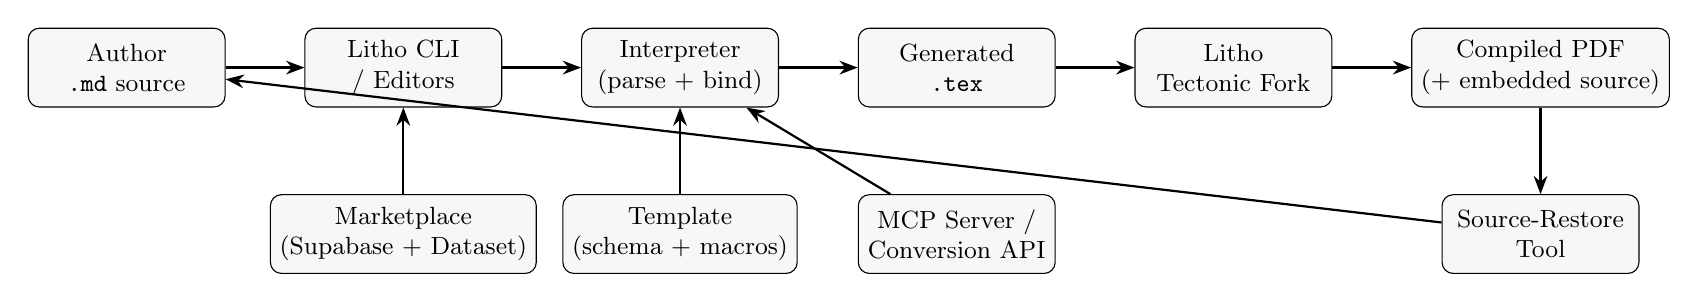
\begin{tikzpicture}[
      node distance=1.1cm and 1cm,
      box/.style={draw, rounded corners, minimum width=2.5cm, minimum height=1cm, align=center, font=\small, fill=inlineCodeBg},
      arrow/.style={-Stealth, thick}
    ]
    \node[box] (md) {Author\\\texttt{.md} source};
    \node[box, right=of md] (cli) {Litho CLI\\/ Editors};
    \node[box, right=of cli] (interp) {Interpreter\\(parse + bind)};
    \node[box, right=of interp] (tex) {Generated\\\texttt{.tex}};
    \node[box, right=of tex] (tectonic) {Litho\\Tectonic Fork};
    \node[box, right=of tectonic] (pdf) {Compiled PDF\\(+ embedded source)};
    \node[box, below=of interp] (template) {Template\\(schema + macros)};
    \node[box, below=of cli] (marketplace) {Marketplace\\(Supabase + Dataset)};
    \node[box, below=of tex] (mcpapi) {MCP Server /\\Conversion API};
    \node[box, below=of pdf] (restore) {Source-Restore\\Tool};

    \draw[arrow] (md) -- (cli);
    \draw[arrow] (cli) -- (interp);
    \draw[arrow] (interp) -- (tex);
    \draw[arrow] (tex) -- (tectonic);
    \draw[arrow] (tectonic) -- (pdf);
    \draw[arrow] (template) -- (interp);
    \draw[arrow] (marketplace) -- (cli);
    \draw[arrow] (mcpapi) -- (interp);
    \draw[arrow] (pdf) -- (restore);
    \draw[arrow] (restore) -- (md);
  \end{tikzpicture}%
  }
  \caption{Litho System Architecture and Author Workflow}
  \label{fig:architecture}
\end{figure}

% ------------------------------------------------------------
\subsection{Tools and Technologies}

\begin{table}[H]
  \centering
  \begin{tabularx}{\textwidth}{>{\raggedright\arraybackslash\hsize=.7\hsize}X >{\raggedright\arraybackslash\hsize=.9\hsize}X >{\raggedright\arraybackslash\hsize=1.4\hsize}X}
    \toprule
    \textbf{Category} & \textbf{Technology} & \textbf{Purpose} \\
    \midrule
    \textbf{Interpreter / CLI}     & Python                              & Grammar, parser, AST, template-binding compiler, and CLI binary \\
    \textbf{LaTeX Compilation}     & Litho-optimized fork of Tectonic~\cite{ref6} & Trimmed, precompiled LaTeX engine invoked by the interpreter \\
    \textbf{VS Code Tooling}       & TypeScript, VS Code Extension API   & Syntax highlighting, snippets, and IntelliSense \\
    \textbf{Other Editor Plugins}  & Vimscript/Lua, Emacs Lisp, IntelliJ Platform SDK & Native Markdown-preview rendering plugins for Vim/Neovim, Emacs, JetBrains IDEs \\
    \textbf{Syntax Highlighting}   & TextMate grammar                    & Static and template-generated highlighting rules \\
    \textbf{Marketplace Web App}   & Next.js                             & Template browsing, publishing, in-browser conversion, AI authoring, and source-restore UI \\
    \textbf{Backend / Database}    & Supabase (Postgres, Auth, Storage)  & Publisher accounts, template metadata, file storage, and template dataset \\
    \textbf{MCP Server / API}      & Python, FastAPI, Model Context Protocol SDK & AI-assistant and third-party webhook access to build/validate/template/extract-source (PDF-to-Markdown reverse) operations \\
    \textbf{PDF Metadata}          & PDF/XMP metadata fields             & Embedding and restoring the original Markdown source from a compiled PDF \\
    \textbf{Markdown Baseline}     & CommonMark~\cite{ref1}              & Base grammar the Litho dialect extends \\
    \textbf{Testing}               & \texttt{pytest}, \texttt{vitest}    & Interpreter, MCP/API, and extension/web app tests \\
    \textbf{Package Distribution}  & PyPI, npm, AUR, VS Code Marketplace, JetBrains Marketplace & CLI, extension, and plugin distribution \\
    \textbf{CI/CD}                 & GitHub Actions                      & Automated build, test, and release pipelines across all package managers \\
    \textbf{Documentation}         & Fumadocs                            & Author-facing (multi-editor setup) and template-author-facing documentation \\
    \textbf{Community}             & GitHub Discussions, Discourse       & Community forum and discussion infrastructure \\
    \bottomrule
  \end{tabularx}
  \caption{Tools and Technologies}
  \label{tab:tools}
\end{table}

% ------------------------------------------------------------
\subsection{Project Timeline}

\begin{table}[H]
  \centering
  \begin{tabularx}{\textwidth}{L c c}
    \toprule
    \textbf{Task / Phase} & \textbf{Start Month} & \textbf{End Month} \\
    \midrule
    \textbf{Phase 1: Language Foundation \& LaTeX Backend} & \textbf{Sep 2026 (M1)} & \textbf{Nov 2026 (M3)} \\
    Research \& Grammar Specification & Sep 2026 (M1) & Sep 2026 (M1) \\
    Parser \& AST & Sep 2026 (M1) & Oct 2026 (M2) \\
    Template-Binding Compiler \& LaTeX Codegen & Oct 2026 (M2) & Nov 2026 (M3) \\
    Litho-Optimized Tectonic Fork (trim, precompile) & Nov 2026 (M3) & Nov 2026 (M3) \\
    \midrule
    \textbf{Phase 2: Author Tooling \& Round-Trip Fidelity} & \textbf{Nov 2026 (M3)} & \textbf{Jan 2027 (M5)} \\
    CLI: init/build/watch/extract-source & Nov 2026 (M3) & Dec 2026 (M4) \\
    Markdown-in-Metadata Embed \& Restore & Dec 2026 (M4) & Dec 2026 (M4) \\
    VS Code Grammar, Snippets \& IntelliSense & Dec 2026 (M4) & Jan 2027 (M5) \\
    Editor Plugins (Vim/Neovim, Emacs, JetBrains) & Jan 2027 (M5) & Jan 2027 (M5) \\
    \midrule
    \textbf{Phase 3: Templates \& Testing} & \textbf{Jan 2027 (M5)} & \textbf{Feb 2027 (M6)} \\
    Flagship Templates (Thesis, IEEE, Book) & Jan 2027 (M5) & Jan 2027 (M5) \\
    Compliance, Regression \& Metadata Round-Trip Test Suite & Jan 2027 (M5) & Feb 2027 (M6) \\
    \midrule
    \textbf{Phase 4: Marketplace, Dataset \& AI Authoring} & \textbf{Feb 2027 (M6)} & \textbf{Apr 2027 (M8)} \\
    Publisher CLI Commands & Feb 2027 (M6) & Feb 2027 (M6) \\
    Marketplace Web App \& Supabase Integration & Feb 2027 (M6) & Mar 2027 (M7) \\
    In-Browser Converter \& Source-Restore Tool & Mar 2027 (M7) & Mar 2027 (M7) \\
    Template Dataset Curation \& AI-Authoring Flow & Mar 2027 (M7) & Apr 2027 (M8) \\
    \midrule
    \textbf{Phase 5: MCP, API \& Community} & \textbf{Apr 2027 (M8)} & \textbf{May 2027 (M9)} \\
    MCP Server (build/validate/template) & Apr 2027 (M8) & Apr 2027 (M8) \\
    Conversion API \& Webhooks & Apr 2027 (M8) & May 2027 (M9) \\
    Community Forum \& GitHub Discussions Setup & May 2027 (M9) & May 2027 (M9) \\
    \midrule
    \textbf{Phase 6: Documentation \& Release} & \textbf{May 2027 (M9)} & \textbf{May 2027 (M9)} \\
    Documentation (Author, Template-Author, Multi-Editor Setup) & May 2027 (M9) & May 2027 (M9) \\
    CI/CD \& Multi-Package-Manager Distribution & May 2027 (M9) & May 2027 (M9) \\
    Final Review \& Submission & May 2027 (M9) & May 2027 (M9) \\
    \bottomrule
  \end{tabularx}
  \caption{Project Timeline Definition (September 2026 -- May 2027)}
  \label{tab:timeline}
\end{table}

\begin{figure}[H]
  \centering
  \resizebox{\textwidth}{!}{%
  \begin{ganttchart}[
      hgrid,
      vgrid,
      x unit=1.2cm,
      y unit chart=0.65cm,
      y unit title=0.75cm,
      title height=1,
      bar/.append style={fill=blue!25, draw=blue!50!black},
      group/.append style={fill=blue!45, draw=blue!70!black},
      bar height=0.6,
      bar label font=\small,
      title label font=\small,
      group label font=\small\bfseries,
  ]{1}{12}

    % Month titles
    \gantttitle{Project Timeline (August 2026 -- July 2027)}{12} \\
    \gantttitle{M1}{1} \gantttitle{M2}{1} \gantttitle{M3}{1} \gantttitle{M4}{1}
    \gantttitle{M5}{1} \gantttitle{M6}{1} \gantttitle{M7}{1} \gantttitle{M8}{1}
    \gantttitle{M9}{1} \gantttitle{M10}{1} \gantttitle{M11}{1} \gantttitle{M12}{1} \\

    % Language Foundation group
    \ganttgroup{Language Foundation \& LaTeX Backend}{1}{3} \\
    \ganttbar{Grammar Specification}{1}{1} \\
    \ganttbar{Parser \& AST}{1}{2} \\
    \ganttbar{Compiler, Codegen \& Tectonic Fork}{2}{3} \\

    % Author Tooling group
    \ganttgroup{Author Tooling \& Round-Trip Fidelity}{3}{6} \\
    \ganttbar{CLI \& Metadata Embed/Restore}{3}{4} \\
    \ganttbar{VS Code Grammar, Snippets \& IntelliSense}{4}{5} \\
    \ganttbar{Editor Plugins (Vim, Emacs, JetBrains)}{5}{6} \\

    % Templates & Testing group
    \ganttgroup{Templates \& Testing}{6}{7} \\
    \ganttbar{Flagship Templates}{6}{6} \\
    \ganttbar{Test Suite}{6}{7} \\

    % Marketplace group
    \ganttgroup{Marketplace, Dataset \& AI Authoring}{7}{9} \\
    \ganttbar{Publisher CLI \& Web App}{7}{8} \\
    \ganttbar{Converter, Source-Restore \& AI Flow}{8}{9} \\

    % MCP/API/Community group
    \ganttgroup{MCP, API \& Community}{9}{10} \\
    \ganttbar{MCP Server \& Conversion API}{9}{10} \\
    \ganttbar{Community Forum Setup}{10}{10} \\

    % Docs & Release group
    \ganttgroup{Docs \& Release}{10}{12} \\
    \ganttbar{Documentation (All Editors)}{10}{11} \\
    \ganttbar{CI/CD \& Multi-Manager Release}{11}{12}

  \end{ganttchart}%
  }
  \caption{Litho Project Timeline}
  \label{fig:timeline}
\end{figure}


% ============================================================
%              CHAPTER 3: TEAM AND WORKFLOW
% ============================================================
\section{Chapter 3: Team and Workflow}

% ------------------------------------------------------------
\subsection{Team Roles and Responsibilities}

The project is divided along the eight components described in Section 2.3, with each member owning a primary set of components while contributing to testing and documentation across the whole system. Table~\ref{tab:roles} summarizes primary ownership; in practice, the language grammar and template schema are treated as a shared contract that all four members review before changes land, since the interpreter, CLI, editor tooling, MCP/API, and marketplace all depend on it.

\begin{table}[H]
  \centering
  \begin{tabularx}{\textwidth}{l L}
    \toprule
    \textbf{Member} & \textbf{Primary Ownership} \\
    \midrule
    Rabia Nadeem & Litho grammar specification, parser, AST, and metadata embed/restore (Python) \\
    Abaidullah Bhatti & Template-binding compiler, LaTeX code generator (Python), and the Litho-optimized Tectonic build configuration \\
    Abdul Rahman & Core Markdown-to-PDF converter and authoring CLI (the existing, in-use tool), the publisher-facing CLI commands, and the flagship templates \\
    Sohaib Shaukat & VS Code extension and other-editor plugins (grammar, snippets, IntelliSense), and the marketplace web application (Next.js, Supabase, dataset, AI authoring, converter) \\
    \bottomrule
  \end{tabularx}
  \caption{Team Roles and Primary Ownership}
  \label{tab:roles}
\end{table}

% ------------------------------------------------------------
\subsection{Development Workflow}

The team follows a trunk-based Git workflow: all work happens on short-lived feature branches merged into \texttt{main} through pull requests, gated by the GitHub Actions CI pipeline (Section 2.4) running the interpreter's unit tests, the extension and plugin test suites, the MCP/API test suite, and, where applicable, a golden-file PDF regression and metadata round-trip check before a merge is permitted. Each of the six project phases in Table~\ref{tab:timeline} closes with a milestone review against its stated deliverables before the next phase begins, and weekly meetings with the supervisor are used to review progress and surface blockers.

Task tracking uses GitHub Issues and a project board organized by the same phase structure as the timeline, so that the full feature set documented in Section 2.1 remains visible and auditable throughout development rather than being agreed once and forgotten.

% ------------------------------------------------------------
\subsection{Risk Management}

\begin{table}[H]
  \centering
  \begin{tabularx}{\textwidth}{L l L}
    \toprule
    \textbf{Risk} & \textbf{Likelihood} & \textbf{Mitigation} \\
    \midrule
    Grammar design churn late in the project forces rework in the compiler and editor tooling & Medium & Freeze the core grammar at the end of Phase 1 (M3); route further syntax needs through template-level extension points rather than core grammar changes \\
    Tectonic fork maintenance burden (upstream drift, missing packages, platform-specific failures) & Medium & Evaluate package coverage against the flagship templates early in Phase 1; track upstream Tectonic changes and re-baseline the fork at the start of each later phase \\
    Twelve-month scope across eight components strains a four-person team & High & The phase-gated timeline (Table~\ref{tab:timeline}) and per-member ownership (Table~\ref{tab:roles}) sequence work so each component is built once its dependencies exist; weekly reviews re-balance member load across phases if one component slips \\
    Marketplace security (arbitrary LaTeX macros in shared templates, MCP/API abuse) & Medium & Sandbox template compilation, restrict templates to a declarative schema plus vetted macro packages, and rate-limit the conversion API and webhooks \\
    Team member availability during exam periods & Low & Timeline built with buffer between phases; task board allows work to be reassigned across members within a phase \\
    \bottomrule
  \end{tabularx}
  \caption{Risk Register}
  \label{tab:risks}
\end{table}

% ------------------------------------------------------------
\subsection{Expected Outcomes}

By the end of the project, the team expects to deliver a working \texttt{litho} CLI and interpreter capable of compiling the extended Markdown dialect against any of the three flagship templates into a publication-quality PDF via the Litho-optimized Tectonic fork, with the original source losslessly recoverable from any compiled PDF's metadata; a published VS Code extension plus companion Vim/Neovim, Emacs, and JetBrains rendering plugins, offering syntax highlighting, snippets, and IntelliSense for both the core language and template-declared shortcodes; a functioning template marketplace supporting publishing (including unified university and company ``house'' templates), in-browser conversion, AI-assisted template authoring and usage (grounded in each template's JSON manifest and SKILLS.md), and PDF source-restoration; a working MCP server and conversion API/webhook so AI assistants and third-party Markdown sites can invoke Litho directly -- including the PDF-to-Markdown \texttt{extract-source} operation that lets an AI recover a document without burning input tokens; and active GitHub Discussions and community-forum infrastructure. Success is evaluated primarily against the regression and metadata round-trip test suite (Section 2.1) and a small usability evaluation in which authors unfamiliar with LaTeX produce a formatted document using Litho and a flagship template, measured against the objectives in Section 1.4.

% ============================================================
%                      REFERENCES
% ============================================================
\clearpage
\begin{thebibliography}{9}

\bibitem{ref1}
CommonMark Spec. \textit{CommonMark: A Strongly Defined, Highly Compatible Specification of Markdown}. \url{https://commonmark.org/}.

\bibitem{ref2}
L. Lamport. \textit{\LaTeX{}: A Document Preparation System}, 2nd ed. Addison-Wesley, 1994.

\bibitem{ref3}
J. MacFarlane. \textit{Pandoc: A Universal Document Converter}. \url{https://pandoc.org/}.

\bibitem{ref4}
Posit, PBC. \textit{Quarto: An Open-Source Scientific and Technical Publishing System}. \url{https://quarto.org/}.

\bibitem{ref5}
Typst GmbH. \textit{Typst: A New Markup-Based Typesetting System}. \url{https://typst.app/}.

\bibitem{ref6}
Tectonic Project. \textit{Tectonic: A Modernized, Complete, Self-Contained \TeX{}/\LaTeX{} Engine}. \url{https://tectonic-typesetting.github.io/}.

\bibitem{ref7}
A. Rahman. \textit{abdxdev/markdown-latex-pdf-builder: The Litho Markdown-to-PDF converter and CLI}. \url{https://github.com/abdxdev/markdown-latex-pdf-builder}.

\end{thebibliography}

\end{document}
